% Provenance (never printed): see sources/outline_sources.md (Year 2: anatexis, migmatites,
% granite types and their sources). Wet granite solidus from Stern and Wyllie (1981) and
% Boettcher and Wyllie (1968); dehydration-melting brackets from Patino Douce and Harris
% (1998), Berger and Kalt (1999), Skjerlie and Johnston (1996); water solubility from Holtz
% et al. (1995); migmatite terms from the IUGS-SCMR proposal and BGS RR 99-02; aluminosity
% after Shand (as given by Moyen et al. 2017); figure data in figdata/bachelor-2/anatexis.py
% (paths from ptpaths.py); exercise and problem values in the Book 4 scratch calculator
% calc/ch12.py.
\chapter{भूपर्पटी का गलन: मिग्मेटाइट और ग्रेनाइट}\label{ch:b2:crustal-melting}

ग्रेनाइट ही महाद्वीपों को हल्का बनाता है, और प्रावार उसे सीधे नहीं बना सकता: \omterm{def:b2:mantle-melting:peridotites}{पेरिडोटाइट}
के गलित बेसाल्ट होते हैं। अधिकांश ग्रेनाइट महाद्वीपीय भूपर्पटी का स्वयं पिघलना है।
जब किसी मोटी हुई पर्वत-जड़ गर्म होती है, जब बेसाल्ट भूपर्पटी के नीचे जमा होता है, या जब कोई गर्म
चट्टान ऊपर उठती है और उसका दाब गिरता है, तब गहरी भूपर्पटी के अभ्रक और एम्फ़ीबोल
अपना जल छोड़ देते हैं, कणों के बीच एक ग्रेनाइटी द्रव प्रकट होता है, और चट्टान एक
\omterm{def:b2:crustal-melting:migmatite}{मिग्मेटाइट} बन जाती है, आधी कायांतरी, आधी आग्नेय। यह अध्याय उस द्रव का उसकी पहली
झिल्लियों से उस \omterm{def:b2:magma-emplacement:bodies}{प्लूटॉन} तक अनुसरण करता है जिसे वह बना सकता है, और किसी ग्रेनाइट के रसायन में वह चट्टान पढ़ता है जिससे वह
आया।

\begin{recall}
\textbf{पुस्तक 2 (उच्च माध्यमिक) से}: ग्रेनाइट, ग्रेनिटॉइड और ग्रैनोडायोराइट; फ़ेल्सिक और मैफ़िक
चट्टानें; पर्वत-पट्टियों की जड़ें। \textbf{पुस्तक 3 (स्नातक वर्ष 1) से}: भूपर्पटी में रेडियोजनिक ऊष्मा-उत्पादन;
सिलिकेटों का जल-अपघटन और मृत्तिका खनिज। \textbf{रसायन-विज्ञान की पुस्तकों से}: द्विघटकी तंत्र का सॉलिडस और लिक्विडस,
मोलर द्रव्यमान और पदार्थ की मात्रा। \textbf{\cref{ch:b2:magma-emplacement}
से}: \omterm{def:b2:magma-emplacement:bodies}{डाइक}, \omterm{def:b2:magma-emplacement:bodies}{प्लूटॉन} और \omterm{def:b2:magma-emplacement:ascent}{डायापिर}। \textbf{\cref{ch:b2:mantle-melting}
से}: \omterm{def:b2:mantle-melting:melting}{आंशिक गलन}, \omterm{def:b2:mantle-melting:peritectic}{असर्वांगसम गलन} और \omterm{def:b2:mantle-melting:melting}{विसंपीडन
गलन}। \textbf{\cref{ch:b2:metamorphic-facies} से}: \omterm{def:b2:metamorphic-facies:protoliths}{मेटापेलाइट}, किसी अभिक्रिया की \omterm{def:b2:metamorphic-facies:clapeyron}{क्लेपेरॉन
ढलान} और संलक्षणियाँ। \textbf{\cref{ch:b2:pt-paths} से}: \omterm{def:b2:pt-paths:ptt}{P--T--t पथ} और
भूपर्पटी का मोटा होने वाला मॉडल।
\end{recall}

\section{भूपर्पटी क्यों पिघलती है}\label{sec:b2:crustal-melting:why}

इसके लिए शब्द पुराना और सीधा-सादा है।

\begin{definition}[ऐनाटेक्सिस]\label{def:b2:crustal-melting:anatexis}
\emph{ऐनाटेक्सिस}\index{ऐनाटेक्सिस} किसी चट्टान का गलन है, गलन की मात्रा जो भी हो;
व्यवहार में यह शब्द महाद्वीपीय भूपर्पटी के \omterm{def:b2:mantle-melting:melting}{आंशिक गलन} के लिए प्रयुक्त होता है।
\end{definition}
% ledger: scmr:migmatite

\subsection*{आर्द्र सॉलिडस}

ग्रेनाइट निम्न तापमान पर तभी पिघलता है जब वह गीला हो। स्टर्न और वायली ने सिएरा नेवादा \omterm{def:b2:magma-emplacement:bodies}{बैथोलिथ} के एक बायोटाइट
ग्रेनाइट को अतिरिक्त जल के साथ पिघलाया: पहला द्रव
\qty{680}{\celsius} पर \qty{2}{kbar} पर और \qty{620}{\celsius} पर \qty{10}{kbar} पर प्रकट हुआ, और
\qty{2}{kbar} पर पूरी चट्टान सॉलिडस से केवल \qty{35}{\celsius} ऊपर ही पिघल गई, पर
\qty{10}{kbar} पर उससे \qty{105}{\celsius} ऊपर। उसी ग्रेनाइट ने, जिसका पहले
बोएचर और वायली ने अध्ययन किया था, \qty{605}{\celsius} पर \qty{15.3}{kbar} पर पिघलना शुरू किया; लगभग
\qty{17}{kbar} पर उसका प्लैजियोक्लेज़ जेडाइट और क्वार्ट्ज़ में टूट गया, और वहाँ से सॉलिडस
फिर ऊपर मुड़ा, \qty{670}{\celsius} पर \qty{27}{kbar} तक पहुँचते हुए।
% ledger: sw81:wet-solidus, bw68:wet-solidus

आर्द्र सॉलिडस दाब बढ़ने पर गिरता है, जो शुष्क सॉलिडस का उलटा है। कारण यह है कि
जल कहाँ जाता है। मुक्त जल कम घनत्व का तरल है; गलित में घुलकर वह बहुत
कम जगह घेरता है: होल्त्ज़ और सहकर्मियों ने ग्रेनाइटी गलित में उसका आंशिक मोलर आयतन
लगभग \qtyrange{10}{12}{\cubic\centi\metre\per\mole} पाया, जबकि कमरे की दशाओं में द्रव जल के लिए यह \qty{18}{\cubic\centi\metre\per\mole}
है और गर्म तरल के लिए इससे अधिक। गलन-अभिक्रिया
\[\text{क्वार्ट्ज़} + \text{फ़ेल्डस्पार} + \ce{H2O}\ (\text{तरल}) \longrightarrow
\text{जलयोजित गलित}\]
इसलिए ऋणात्मक आयतन-परिवर्तन रखती है, जबकि उसका एन्ट्रॉपी-परिवर्तन, किसी भी गलन की तरह,
धनात्मक है: क्लेपेरॉन संबंध (\cref{ch:b2:metamorphic-facies}) से उसकी ढलान
$\mathrm{d}P/\mathrm{d}T = \Delta S/\Delta V$ ऋणात्मक है। दाब गलित में और अधिक जल भी
जाने देता है: \qty{800}{\celsius} पर हैप्लोग्रेनाइट गलित के लिए संतृप्ति-मात्रा
\qty{2.80}{\percent} द्रव्यमान से, \qty{0.5}{kbar} पर, बढ़कर \qty{9.97}{\percent} हो जाती है,
\qty{5}{kbar} पर, और \qty{13.82}{\percent}, \qty{8}{kbar} पर, यानी लगभग \qty{1.27}{\percent} अधिक
प्रति किलोबार, 3 और \qty{8}{kbar} के बीच।
% ledger: holtz95:solubility

\begin{omfigure}
\centering
\begin{tikzpicture}
\begin{axis}[omrecord, width=0.5\linewidth, height=4.8cm,
  xmin=0, xmax=9, ymin=0, ymax=15, xlabel={$P$ (\unit{kbar})},
  ylabel={गलित में \ce{H2O} (\unit{\percent})},
  tick label style={font=\scriptsize}, label style={font=\small}]
\addplot[only marks, mark=*, mark size=1.6pt, blue!70!black]
  table[x=P_kbar, y=H2O_wt] {figdata/out/bachelor-2-anatexis-water.dat};
\addplot[thick, red!75!black] table[x=P_kbar, y=H2O_wt] {figdata/out/bachelor-2-anatexis-waterfit.dat};
\end{axis}
\end{tikzpicture}
\par\smallskip{\small वह जल जो कोई हैप्लोग्रेनाइट गलित \qty{800}{\celsius} पर घोल सकता है
(मापे गए बिंदु); लाल: 3 से
\qty{8}{kbar} तक के बिंदुओं से होकर न्यूनतम-वर्ग रेखा, ढलान \qty{1.26}{\percent} प्रति किलोबार।}
\end{omfigure}
% ledger: holtz95:solubility

पर गहरी भूपर्पटी में मुक्त जल कम होता है: गर्म की जा चुकी कायांतरी चट्टान
\cref{ch:b2:metamorphic-facies} की निर्जलीकरण अभिक्रियाओं द्वारा अपना अधिकांश रंध्र-जल पहले ही
बाहर निकाल चुकी होती है। उसका जल अब अभ्रकों और एम्फ़ीबोलों में बंद है। तब गलन को
इन खनिजों के स्वयं टूटने की प्रतीक्षा करनी पड़ती है।

\begin{definition}[तरल-उपस्थित गलन और निर्जलीकरण गलन]\label{def:b2:crustal-melting:reactions}
\emph{तरल-उपस्थित गलन}\index{तरल-उपस्थित गलन} (या जल-प्रवाहित गलन) मुक्त जलीय तरल की
उपस्थिति में, आर्द्र सॉलिडस पर या उसके निकट, होने वाला गलन है; उत्पन्न गलित
तरल की आपूर्ति से सीमित होता है। \emph{निर्जलीकरण गलन}\index{निर्जलीकरण गलन}
(तरल-अनुपस्थित गलन) किसी जलयोजित खनिज, अभ्रक या
एम्फ़ीबोल, का क्वार्ट्ज़ और फ़ेल्डस्पार के साथ, बिना किसी मुक्त तरल के, \omterm{def:b2:mantle-melting:peritectic}{असर्वांगसम गलन} है: खनिज का जल
गलित में चला जाता है, और नए निर्जल खनिज (पेरिटेक्टिक पोटैशियम फ़ेल्डस्पार, ऐलुमिनोसिलिकेट,
गार्नेट, कॉर्डिएराइट, ऑर्थोपाइरॉक्सीन) उसके बगल में उगते हैं।
\end{definition}
% ledger: pj98:productivity, koester02:melting, pdh98:himalaya

प्रयोग तय करते हैं कि हर जलयोजित खनिज कहाँ जगह छोड़ता है। हिमालय की मस्कोवाइट शिस्टों में
पातिन्यो डूस और हैरिस ने पाया कि \omterm{def:b2:crustal-melting:reactions}{निर्जलीकरण गलन} 750 से
\qty{800}{\celsius} पर, 6 और \qty{10}{kbar} के बीच, शुरू होता है; उन्हीं चट्टानों में जल मिलाने पर
सॉलिडस नीचे आया पर ट्रॉन्डजेमाइटी गलित मिले जो \omterm{def:b2:crustal-melting:leucogranite}{ल्यूकोग्रेनाइटों} से भिन्न थे। एक अर्ध-पेलाइटी नाइस
अपने फ़ेंजाइटी मस्कोवाइट के कारण लगभग \qty{700}{\celsius} पर पिघलने लगा, पर उसने
\qty{9}{\percent} से कम गलित उत्पन्न किया; \qty{800}{\celsius} से ऊपर बायोटाइट और
कॉर्डिएराइट के टूटने से आयतन के अनुसार 10 से \qty{63}{\percent} गलित मिला। बायोटाइट का \omterm{def:b2:crustal-melting:reactions}{निर्जलीकरण गलन}
बवेरियाई वन (बायरिशे वाल्ड) के \omterm{def:b2:crustal-melting:migmatite}{मिग्मेटाइटों} में 800 से \qty{850}{\celsius} और 0.5 से \qty{0.7}{GPa} पर हुआ,
और एम्फ़ीबोल 875
और \qty{925}{\celsius} के बीच, 10 से \qty{12.5}{kbar} पर, आयतन के अनुसार लगभग \qty{25}{\percent} गलित जोड़ता है। क्रम जल की पकड़ का क्रम है:
पहले मस्कोवाइट, फिर बायोटाइट, अंत में एम्फ़ीबोल।
% ledger: pdh98:himalaya, koester02:melting, bk99:migmatites, sj96:amphibole, moyen17:aluminosity

\begin{proposition}[जल से सीमित गलन-अंश]\label{prop:b2:crustal-melting:water}
बिना किसी मुक्त तरल के \omterm{def:b2:crustal-melting:reactions}{निर्जलीकरण गलन} में, यदि किसी चट्टान में द्रव्यमान-अंश $X$ का
ऐसा जलयोजित खनिज है जिसमें द्रव्यमान-अंश $w$ जल है, और यदि यह सारा जल ऐसे
गलित में जाता है जिसमें द्रव्यमान-अंश $c$ जल है, तो गलित का द्रव्यमान-अंश है
\[F = \frac{X\,w}{c}.\]
क्योंकि $c$ गलन के दाब और तापमान पर संतृप्ति-मात्रा $c_{\mathrm{sat}}$ से अधिक नहीं हो
सकता, $F \ge X\,w/c_{\mathrm{sat}}$: गलित जितना कम जल रखता है,
वही अभ्रक उतना अधिक गलित बनाता है।
\end{proposition}

\begin{proof}
चट्टान के प्रति किलोग्राम खनिज $X\,w$ किलोग्राम जल छोड़ता है। कोई तरल प्रावस्था न होने
और ठोसों में कोई जल न बचने पर, वह सब गलित में है, जिसका द्रव्यमान $F$ अपने में $c\,F$
किलोग्राम जल रखता है: $c\,F = X\,w$। चूँकि $c \le c_{\mathrm{sat}}$, $F = Xw/c \ge
Xw/c_{\mathrm{sat}}$।
\end{proof}

\qty{398.3}{\gram\per\mole} मोलर द्रव्यमान वाला मस्कोवाइट, \ce{KAl3Si3O10(OH)2}, दो
हाइड्रॉक्सिल समूह रखता है, जो जल के एक अणु के तुल्य है, यानी उसके द्रव्यमान का \qty{4.52}{\percent}।
अतः \qty{20}{\percent} मस्कोवाइट वाली शिस्ट के पास देने के लिए \qty{9.0}{\gram} जल
प्रति किलोग्राम है; \qty{6}{\percent} पर घुलकर यह \qty{150}{\gram}
गलित बनाता है। अभ्रक बजट तय करते हैं, इसीलिए उर्वर भूपर्पटी, यानी वह भूपर्पटी जो आसानी से पिघलती है,
अभ्रक से समृद्ध होती है: उनमें सबसे पहले \omterm{def:b2:metamorphic-facies:protoliths}{मेटापेलाइट}।

\begin{omfigure}
\centering
\begin{tikzpicture}
\begin{axis}[omrecord, width=0.8\linewidth, height=7cm,
  xmin=500, xmax=1000, ymin=0, ymax=20, xlabel={$T$ (\unit{\celsius})}, ylabel={$P$ (\unit{kbar})},
  tick label style={font=\scriptsize}, label style={font=\small}, clip=false]
\addplot[fill=orange!35, draw=orange!70!black] coordinates {(750,6) (800,6) (800,10) (750,10) (750,6)};
\addplot[fill=red!25, draw=red!70!black] coordinates {(800,5) (850,5) (850,7) (800,7) (800,5)};
\addplot[fill=green!25, draw=green!50!black] coordinates {(875,10) (925,10) (925,12.5) (875,12.5) (875,10)};
\node[font=\scriptsize, orange!50!black, align=center] at (axis cs:775,8) {मस्को-\\वाइट};
\node[font=\scriptsize, red!60!black] at (axis cs:825,4.4) {बायोटाइट};
\node[font=\scriptsize, green!35!black, anchor=west] at (axis cs:927,11.25) {एम्फ़ीबोल};
\addplot[very thick, blue!70!black, mark=*, mark size=1.5pt]
  table[x=T_C, y=P_kbar] {figdata/out/bachelor-2-anatexis-solidi.dat};
\node[font=\scriptsize, blue!70!black, anchor=west] at (axis cs:612,15.6) {ग्रेनाइट का आर्द्र सॉलिडस};
\addplot[thick, black, postaction={decorate}, decoration={markings,
  mark=at position 0.3 with {\arrow{>}}, mark=at position 0.75 with {\arrow{>}}}]
  table[x=T_C, y=P_kbar, restrict x to domain=500:1000,
  restrict expr to domain={\thisrow{t_Myr}}{0:100}] {figdata/out/bachelor-2-anatexis-path35.dat};
\node[font=\scriptsize, anchor=north] at (axis cs:560,4.2) {\qty{35}{km} वाली चट्टान};
\addplot[thick, dashed, black, postaction={decorate}, decoration={markings,
  mark=at position 0.3 with {\arrow{>}}, mark=at position 0.7 with {\arrow{>}}}]
  table[x=T_C, y=P_kbar, restrict x to domain=500:1000,
  restrict expr to domain={\thisrow{t_Myr}}{0:100}] {figdata/out/bachelor-2-anatexis-path70.dat};
\node[font=\scriptsize, anchor=south] at (axis cs:760,19.4) {मोटी हुई भूपर्पटी का आधार};
\end{axis}
\end{tikzpicture}
\par\smallskip{\small भूपर्पटी कहाँ पिघलती है। नीला: अतिरिक्त जल के साथ एक बायोटाइट ग्रेनाइट का
सॉलिडस (मापे गए बिंदु, सीधे खंडों से जुड़े)। बक्से: वे दशाएँ जिन पर
मस्कोवाइट, बायोटाइट और एम्फ़ीबोल का \omterm{def:b2:crustal-melting:reactions}{निर्जलीकरण गलन} प्रयोगों में और
\omterm{def:b2:crustal-melting:migmatite}{मिग्मेटाइटों} में देखा गया। काला: \cref{ch:b2:pt-paths} के मोटा होने वाले मॉडल से परिकलित
पथ; चढ़ाव के बाद \qty{35}{km} पर पहुँचने वाली चट्टान (ठोस रेखा) कभी
आर्द्र सॉलिडस तक नहीं पहुँचती, जबकि मोटी हुई भूपर्पटी का आधार (डैश रेखा)
\qty{900}{\celsius} पार कर जाता है। दोनों पथ पहले 100 मिलियन वर्षों के लिए, अपरदन रुकने तक,
खींचे गए हैं।}
\end{omfigure}
% ledger: sw81:wet-solidus, bw68:wet-solidus, pdh98:himalaya, bk99:migmatites, sj96:amphibole, et84:ptt

\subsection*{ऊष्मा कहाँ से आती है}

ऊपर का चित्र समस्या प्रस्तुत करता है: भूपर्पटी केवल वहीं पिघलती है जहाँ वह लगभग
\qty{700}{\celsius} से अधिक गर्म हो, जबकि \cref{ch:b2:pt-paths} के मॉडल का स्थायी जियोथर्म
\qty{35}{km} भूपर्पटी के आधार पर केवल \qty{595}{\celsius} तक पहुँचता है। तीन रास्ते
निर्जलीकरण-गलन अभिक्रियाओं से आगे ले जाते हैं।

\emph{मोटा होना और रेडियोजनिक ऊष्मा।} \cref{ch:b2:pt-paths} के मॉडल में, चढ़ाव से दोगुनी हुई
भूपर्पटी भीतर से गर्म होती है; मध्य-भूपर्पटीय गहराई पर पहुँचने वाली चट्टान का शिखर
\qty{593}{\celsius} पर है और वह कभी नहीं पिघलती, पर मोटी हुई भूपर्पटी का आधार लगभग 31 मिलियन वर्षों बाद
\qty{800}{\celsius} और लगभग 56 के बाद \qty{900}{\celsius} पार कर जाता है, बायोटाइट
अभिक्रिया से आगे। निचली भूपर्पटी का गलन मोटा होने का एक धीमा परिणाम है।
% ledger: et84:ptt

\emph{विसंपीडन।} ठंडा होने से तेज़ी से ऊपर लाई गई गर्म चट्टान
निर्जलीकरण-गलन वक्रों को उच्च-दाब पक्ष से पार करती है। पातिन्यो डूस और हैरिस ने पाया कि
मस्कोवाइट शिस्ट के सॉलिडस का $\mathrm{d}P/\mathrm{d}T$ बायोटाइट शिस्ट के सॉलिडस से छोटा है,
जिससे मस्कोवाइट शिस्ट विसंपीडन पर अधिक आसानी से पिघलती है, और
निष्कर्ष निकाला कि हिमालय के \omterm{def:b2:crustal-melting:leucogranite}{ल्यूकोग्रेनाइट} \omterm{def:b2:metamorphic-facies:protoliths}{मेटापेलाइटों} के \omterm{def:b2:crustal-melting:reactions}{निर्जलीकरण गलन} से
रुद्धोष्म विसंपीडन के दौरान, 6 से \qty{8}{kbar} और 750 से \qty{770}{\celsius} पर, बने।
% ledger: pdh98:himalaya

\emph{नीचे से ऊष्मा।} प्रावार से आया बेसाल्ट जो भूपर्पटी के आधार पर रुक जाता है, अपने साथ
अपनी ऊष्मा और क्रिस्टलन की अपनी गुप्त ऊष्मा लाता है।

\begin{definition}[मैफ़िक अधःस्तरण]\label{def:b2:crustal-melting:underplating}
\emph{मैफ़िक अधःस्तरण}\index{मैफ़िक अधःस्तरण} प्रावार से व्युत्पन्न
बेसाल्टी \omterm{def:b2:magma-emplacement:magma}{मैग्मा} का महाद्वीपीय भूपर्पटी के आधार पर या उसके निकट जमा होना है, जहाँ वह क्रिस्टलित होता है और
अपनी ऊष्मा ऊपर की भूपर्पटी में छोड़ता है।
\end{definition}

उदाहरण के लिए, अंटार्कटिक प्रायद्वीप के रायोलाइटों के लिए अधःस्तरण का सहारा लिया गया,
जहाँ एंडेसाइटी से डेसाइटी \omterm{def:b2:magma-emplacement:magma}{मैग्मा} अधःस्तरण की प्रतिक्रिया में जलयोजित मैफ़िक निचली भूपर्पटी के
गलन से आया; प्रावार के गलित स्वयं भी ग्रेनिटॉइड बना सकते हैं,
क्रिस्टलित होकर या हाल में अधःस्तरित पिंडों को फिर से पिघलाकर।
% ledger: riley01:underplating, moyen17:settings, johansson23:a-type

\begin{proposition}[अधःस्तरण का ऊष्मा-बजट]\label{prop:b2:crustal-melting:heat}
आयतन $V_b$ का बेसाल्ट, जो $T_b$ पर अंतर्वेधित होकर पूरी तरह क्रिस्टलित होता है, प्रति एकांक आयतन
गुप्त ऊष्मा $L_b$ छोड़ता है, और $T_f$ तक ठंडा होता है, भूपर्पटी के आयतन $V_c$ को
$T_c$ से $T_f$ तक ला सकता है और उसके अंश $F$ को पिघला सकता है, जहाँ
\[\frac{V_c}{V_b} = \frac{L_b + C\,(T_b - T_f)}{C\,(T_f - T_c) + F\,L_c},\]
जहाँ $C$ प्रति एकांक आयतन ऊष्मा धारिता है (दोनों चट्टानों के लिए बराबर मानी गई) और $L_c$
प्रति एकांक आयतन भूपर्पटीय गलित की गुप्त ऊष्मा, यदि कोई ऊष्मा न खोई जाए।
\end{proposition}

\begin{proof}
बेसाल्ट द्वारा छोड़ी गई ऊष्मा, $V_b[L_b + C(T_b - T_f)]$, भूपर्पटी द्वारा ली गई ऊष्मा
$V_c[C(T_f - T_c) + F L_c]$ के बराबर है; $V_b$ से और भूपर्पटी वाले कोष्ठक से भाग दीजिए।
\end{proof}

$C = \qty{2.5}{\mega\joule\per\cubic\metre\per\kelvin}$ और
\qty{900}{\mega\joule\per\cubic\metre} की गुप्त ऊष्माओं के साथ, जो \omterm{def:b2:magma-emplacement:magma}{मैग्मा} के लिए प्ररूपी मान हैं,
\qty{1200}{\celsius} से \qty{850}{\celsius} तक ठंडा होता बेसाल्ट अपने आयतन की लगभग ढाई गुनी
भूपर्पटी को \qty{650}{\celsius} से गर्म कर सकता है और उसका पाँचवाँ भाग पिघला सकता है (\cref{exo:b2:crustal-melting:7})।
अधःस्तरण कुशल है, पर स्थानीय: ऊष्मा वहीं जाती है जहाँ बेसाल्ट है।
% ledger: delaney86b4:properties

\section{ऐनाटेक्सिस और मिग्मेटाइट}\label{sec:b2:crustal-melting:migmatites}

कोई आंशिक रूप से पिघली चट्टान, जो अपने गलित के निकलने से पहले जम जाती है, दोनों भागों को साथ-साथ रखती है।

\begin{definition}[मिग्मेटाइट और उसके भाग]\label{def:b2:crustal-melting:migmatite}
\emph{मिग्मेटाइट}\index{मिग्मेटाइट} एक संयुक्त सिलिकेट चट्टान है, जो अनावरण के
पैमाने पर विषमांगी है, और कायांतरी चट्टान जैसे दिखने वाले गहरे भागों और प्लूटोनी रूप वाले हल्के भागों
से बनी है। उसका \emph{ल्यूकोसोम}\index{ल्यूकोसोम} उसका हल्का, क्वार्ट्ज़- और
फ़ेल्डस्पार-समृद्ध भाग है; उसका \emph{मेलानोसोम}\index{मेलानोसोम} उसका गहरा भाग, गहरे
खनिजों से समृद्ध, ल्यूकोसोम का पूरक; उसका \emph{मीसोसोम} मध्यवर्ती
रंग का भाग, जनक चट्टान (\emph{पेलियोसोम}) का कमोबेश परिवर्तित अवशेष।
ल्यूकोसोम और मेलानोसोम मिलकर \emph{नियोसोम} बनाते हैं, यानी नया बना भाग। एक
\emph{मेटाटेक्साइट}\index{मेटाटेक्साइट} वह मिग्मेटाइट है जिसमें अलग-अलग, सुस्पष्ट ल्यूकोसोम,
मीसोसोम और मेलानोसोम हों; एक \emph{डायाटेक्साइट}\index{डायाटेक्साइट} वह है जिसमें हल्के और
गहरे भाग धारियों (श्लीरेन) और प्रेत-जैसी (नेबुलाइटी) संरचनाओं में घुल-मिल जाते हैं।
\end{definition}
% ledger: scmr:migmatite, bgs99:migmatite

परिभाषा जानबूझकर वर्णनात्मक है: कोई \omterm{def:b2:crustal-melting:migmatite}{ल्यूकोसोम} जमा हुआ गलित है, कहीं और से आया
गलित है, या कायांतरी पृथक्करण है, यह एक व्याख्या है। जब वह
गलित होता है, तो \omterm{def:b2:crustal-melting:migmatite}{ल्यूकोसोम} द्रव है और \omterm{def:b2:crustal-melting:migmatite}{मेलानोसोम} वह ठोस अवशेष जो उसने छोड़ा, बायोटाइट,
गार्नेट या कॉर्डिएराइट से समृद्ध: \omterm{def:b2:crustal-melting:migmatite}{मेटाटेक्साइट} \omterm{def:b2:crustal-melting:anatexis}{ऐनाटेक्सिस} के पहले चरण को अंकित करता है, जहाँ
चट्टान का केवल एक भाग पिघला, और \omterm{def:b2:crustal-melting:migmatite}{डायाटेक्साइट} एक आगे के चरण को, जहाँ गहरे खनिज
भी पिघले और गलित अपनी जगह पर रहा।
% ledger: scmr:migmatite

किसी \omterm{def:b2:crustal-melting:migmatite}{मिग्मेटाइट} में कितना गलित होता है? बवेरियाई वन के कॉर्डिएराइट \omterm{def:b2:crustal-melting:migmatite}{मिग्मेटाइटों} में,
जो बायोटाइट के \omterm{def:b2:crustal-melting:reactions}{निर्जलीकरण गलन} से बने, वे \omterm{def:b2:crustal-melting:migmatite}{ल्यूकोसोम} जो शुद्ध पूर्व-गलित हैं, आयतन के अनुसार चट्टान का 20 से
\qty{40}{\percent} बनाते हैं, जो समान दशाओं पर समान चट्टानों पर हुए निर्जलीकरण-गलन प्रयोगों में उत्पन्न
20 से \qty{30}{\percent} के निकट है; जहाँ गलित
हटाया गया, जैसे सबसे अधिक विरूपित प्रकारों में, वहाँ अवशेष पीछे छूट जाता है।
% ledger: bk99:migmatites

\begin{inthefield}[मिग्मेटाइट के अनावरण को पढ़ना]
\omterm{def:b2:crustal-melting:migmatite}{मिग्मेटाइट} के किसी अनावरण पर भूवैज्ञानिक पहले भागों और उनकी ज्यामिति का मानचित्रण करता है: क्या
\omterm{def:b2:crustal-melting:migmatite}{ल्यूकोसोम} पर्णन में स्थित हैं या उसे काटते हैं, क्या उनके साथ गहरी मेलानोक्रेटी किनारी है,
और हर \omterm{def:b2:crustal-melting:migmatite}{ल्यूकोसोम} के लिए कितना \omterm{def:b2:crustal-melting:migmatite}{मेलानोसोम} है। हर लक्षण का एक अर्थ है। अवशिष्ट,
मेलानोक्रेटी चट्टान दर्शाती है कि गलित कहाँ से आया; पतले, छोटे, शाखित \omterm{def:b2:crustal-melting:migmatite}{ल्यूकोसोम}, जिनके साथ
थोड़ा \omterm{def:b2:crustal-melting:migmatite}{मेलानोसोम} हो, अभी शुरू हुए गलन को दर्शाते हैं; पर्णन के समांतर \omterm{def:b2:crustal-melting:migmatite}{ल्यूकोसोम}
दर्शाते हैं कि गलित आधात्री से कहाँ रिसकर इकट्ठा हुआ; परतों से बड़े कोण पर स्थित \omterm{def:b2:crustal-melting:migmatite}{ल्यूकोसोम},
प्रायः गहरी किनारी के बिना, अंत में बने और उन नलिकाओं को दर्शाते हैं जिनसे होकर
गलित निकला। \omterm{def:b2:crustal-melting:migmatite}{मेलानोसोम} और \omterm{def:b2:crustal-melting:migmatite}{ल्यूकोसोम} का ऊँचा अनुपात बताता है कि अधिकांश गलित जा चुका है।
फिर \omterm{def:b2:crustal-melting:migmatite}{ल्यूकोसोम}, \omterm{def:b2:crustal-melting:migmatite}{मेलानोसोम} और मीसोसोम के नमूने विश्लेषण के लिए लिए जाते हैं, ताकि द्रव्यमान-संतुलन
से परखा जा सके कि अनावरण ने गलित खोया या नहीं (\cref{exo:b2:crustal-melting:12})।
\end{inthefield}
% ledger: sawyer01:segregation, bgs99:migmatite, scmr:migmatite

\begin{omfigure}
\centering
\begin{tikzpicture}[x=1cm, y=1cm]
% (a) stromatic
\begin{scope}
\fill[gray!45] (0,0) rectangle (3,3);
\foreach \y in {0.45, 1.25, 2.05, 2.7} {
  \fill[black!70] (0,\y-0.2) .. controls (1,\y-0.15) and (2,\y-0.25) .. (3,\y-0.2)
    -- (3,\y+0.2) .. controls (2,\y+0.15) and (1,\y+0.25) .. (0,\y+0.2) -- cycle;
  \fill[white] (0,\y-0.14) .. controls (1,\y-0.09) and (2,\y-0.19) .. (3,\y-0.14)
    -- (3,\y+0.14) .. controls (2,\y+0.09) and (1,\y+0.19) .. (0,\y+0.14) -- cycle;
}
\draw[thick] (0,0) rectangle (3,3);
\node[font=\small, anchor=north] at (1.5,-0.1) {(क) स्ट्रोमैटिक};
\end{scope}
% (b) agmatitic
\begin{scope}[xshift=3.4cm]
\fill[white] (0,0) rectangle (3,3);
\fill[gray!45, draw=black!70, thick] (0.15,0.15) -- (1.3,0.25) -- (1.2,1.25) -- (0.2,1.1) -- cycle;
\fill[gray!45, draw=black!70, thick] (1.5,0.2) -- (2.85,0.15) -- (2.8,1.0) -- (1.6,1.35) -- cycle;
\fill[gray!45, draw=black!70, thick] (0.2,1.35) -- (1.25,1.5) -- (1.4,2.8) -- (0.15,2.85) -- cycle;
\fill[gray!45, draw=black!70, thick] (1.65,1.6) -- (2.85,1.25) -- (2.85,2.85) -- (1.6,2.8) -- cycle;
\draw[thick] (0,0) rectangle (3,3);
\node[font=\small, anchor=north] at (1.5,-0.1) {(ख) ऐग्मैटाइटी};
\end{scope}
% (c) schlieric
\begin{scope}[xshift=6.8cm]
\fill[white] (0,0) rectangle (3,3);
\foreach \y/\a in {0.5/0.3, 1.1/-0.25, 1.7/0.2, 2.3/-0.3} {
  \draw[black!75, line width=1.4pt] (0.2,\y) .. controls (1,\y+\a) and (1.8,\y-\a) .. (2.8,\y+0.1);
}
\draw[black!60, line width=0.8pt] (0.6,2.75) .. controls (1.4,2.55) .. (2.4,2.8);
\draw[thick] (0,0) rectangle (3,3);
\node[font=\small, anchor=north] at (1.5,-0.1) {(ग) श्लीरेनी};
\end{scope}
% (d) nebulitic
\begin{scope}[xshift=10.2cm]
\fill[white] (0,0) rectangle (3,3);
\shade[inner color=gray!50, outer color=white] (0.9,1.0) ellipse (0.75 and 0.45);
\shade[inner color=gray!45, outer color=white] (2.1,2.1) ellipse (0.7 and 0.4);
\shade[inner color=gray!35, outer color=white] (2.2,0.7) ellipse (0.5 and 0.3);
\draw[thick] (0,0) rectangle (3,3);
\node[font=\small, anchor=north] at (1.5,-0.1) {(घ) नेबुलाइटी};
\end{scope}
\end{tikzpicture}
\par\smallskip{\small \omterm{def:b2:crustal-melting:migmatite}{मिग्मेटाइटों} की चार संरचनाएँ, योजनामूलक (अनावरण-फलक लगभग एक मीटर
चौड़े)। सफ़ेद: \omterm{def:b2:crustal-melting:migmatite}{ल्यूकोसोम}; काला: \omterm{def:b2:crustal-melting:migmatite}{मेलानोसोम}; धूसर: मीसोसोम। (क) स्ट्रोमैटिक: \omterm{def:b2:crustal-melting:migmatite}{ल्यूकोसोम} की
परतें, हर एक गहरी किनारी के साथ, पर्णन के समांतर, मेटाटेक्साइटों में प्ररूपी।
(ख) ऐग्मैटाइटी: कोणीय खंडों के चारों ओर \omterm{def:b2:crustal-melting:migmatite}{ल्यूकोसोम} शिराओं का जाल, जो ब्रेशिया-जैसा
रूप देता है। (ग) श्लीरेनी: \omterm{def:b2:crustal-melting:migmatite}{ल्यूकोसोम} के भीतर गहरे खनिजों की धारियाँ। (घ) नेबुलाइटी: आग्नेय-से दिखने वाले आधार में
पूर्ववर्ती चट्टान की धुँधली प्रेत-छायाएँ; (ग) और (घ)
डायाटेक्साइटों में प्ररूपी हैं।}
\end{omfigure}
% ledger: bgs99:migmatite, scmr:migmatite

\begin{omfigure}
\centering
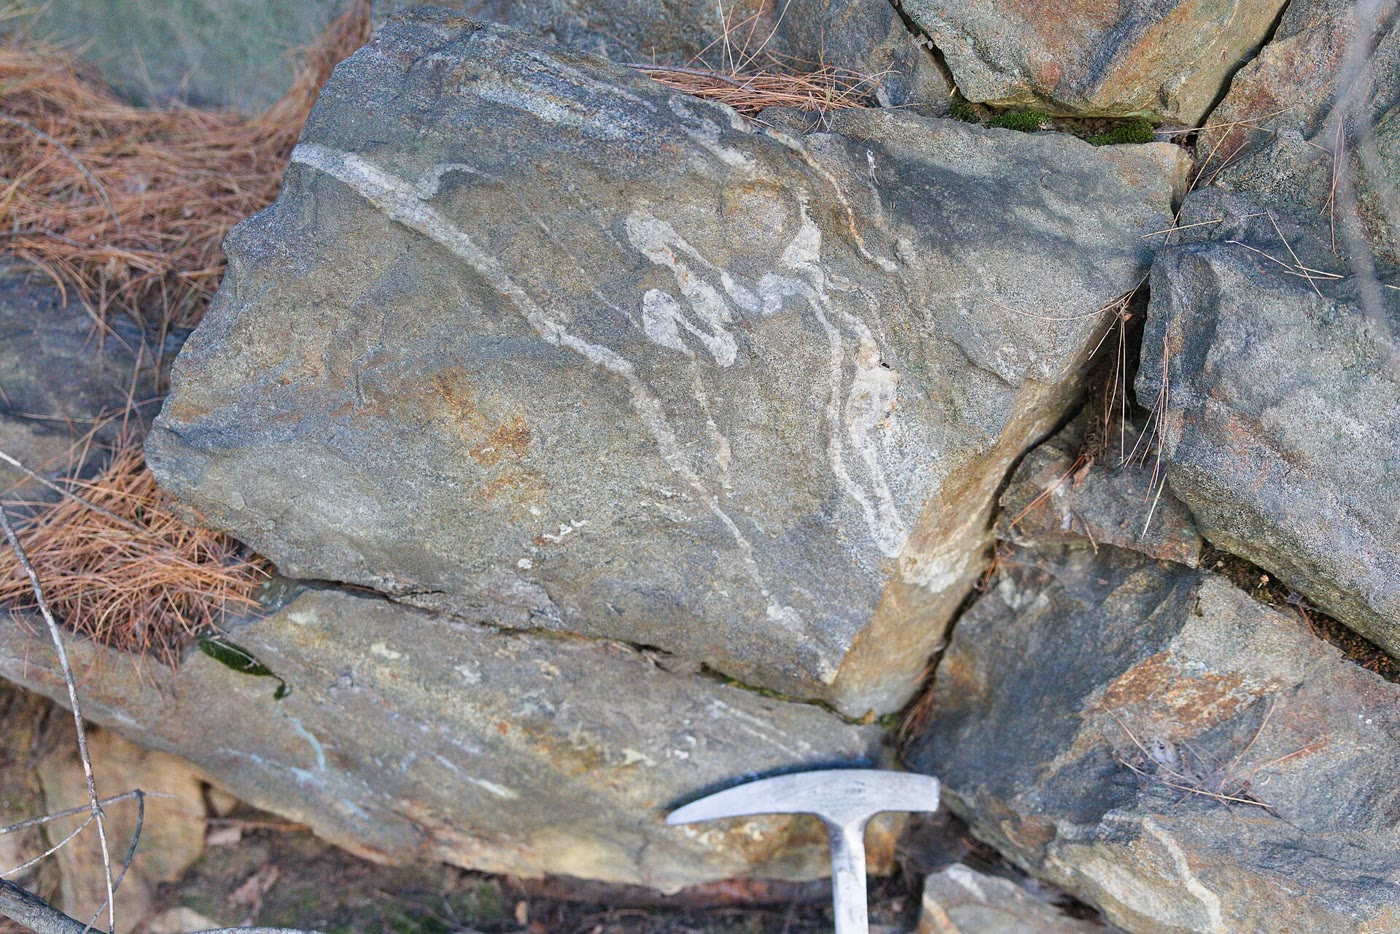
\includegraphics[width=0.62\linewidth]{images/book4/b2-12-migmatite.jpg}
\par\smallskip{\small नैशुआ, न्यू हैम्पशायर में एक \omterm{def:b2:crustal-melting:migmatite}{मिग्मेटाइट}: हल्की \omterm{def:b2:crustal-melting:migmatite}{ल्यूकोसोम} शिराएँ, उन्हें धारण करने वाले धूसर
नाइस के साथ वलित। भूवैज्ञानिक का हथौड़ा पैमाना देता है। फ़ोटो: Kevin M. Gill, CC BY 4.0।}
\end{omfigure}

\section{मिग्मेटाइट से प्लूटॉन तक}\label{sec:b2:crustal-melting:segregation}

कण के पैमाने पर पहला गलित कण-सीमाओं के अनुदिश और छोटे कुंडों में स्थित होता है,
अधिकतर पर्णन के समांतर। छोटा होते हुए भी वह चट्टान को बदल देता है: आंशिक रूप से पिघले ग्रेनाइट
पर प्रयोगों में समुच्चय की सामर्थ्य सॉलिडस और \num{0.07} के \omterm{def:b2:mantle-melting:fraction}{गलन-अंश} के बीच
तेज़ी से गिरती है, जब गलित वाली कण-सीमाएँ जुड़ती हैं, और फिर
गिरती है, परिमाण की लगभग चार कोटियों से, यद्यपि पहले से ही कम मान से, जब क्रिस्टल-ढाँचा
उच्चतर \omterm{def:b2:mantle-melting:fraction}{गलन-अंशों} पर टूट जाता है। इसलिए आंशिक रूप से पिघली भूपर्पटी दुर्बल होती है,
और गलन शुरू होते ही विरूपण वहाँ इकट्ठा हो जाता है। विरूपण बदले में
गलित को चलाता है: वह आधात्री से जुड़ी कण-सीमाओं के अनुदिश पर्णन के समांतर \omterm{def:b2:crustal-melting:migmatite}{ल्यूकोसोमों} में रिसता है,
फिर उसे काटने वाले \omterm{def:b2:crustal-melting:migmatite}{ल्यूकोसोमों} से होकर गलन-परत से बाहर, और
ये \cref{ch:b2:magma-emplacement} के \omterm{def:b2:magma-emplacement:bodies}{डाइकों} में मिल जाते हैं। नीचे का चित्र
स्रोत से \omterm{def:b2:magma-emplacement:bodies}{प्लूटॉन} तक के पथ का सार प्रस्तुत करता है।
% ledger: sawyer01:segregation, rh05:connectivity

\begin{omfigure}
\centering
\begin{tikzpicture}[x=1cm, y=1cm]
\fill[gray!20] (0,0) rectangle (11,1.6);
\fill[gray!8] (0,1.6) rectangle (11,5.2);
\node[font=\scriptsize, anchor=west] at (0.1,0.25) {मिग्मेटाइटी निचली भूपर्पटी (स्रोत)};
\foreach \x in {0.6,1.6,2.6,3.6,4.6,5.6,6.6,7.6,8.6,9.6} {
  \draw[white, line width=2.2pt] (\x,0.65) .. controls (\x+0.3,0.75) and (\x+0.5,0.6) .. (\x+0.8,0.7);
  \draw[white, line width=2.2pt] (\x+0.2,1.2) .. controls (\x+0.45,1.3) and (\x+0.6,1.15) .. (\x+0.85,1.25);
}
\foreach \x in {2.8, 5.2, 7.9} {
  \draw[red!70!black, line width=1.4pt] (\x,1.3) .. controls (\x+0.1,2.2) and (\x-0.1,2.9) .. (5.5,3.65);
}
\fill[pink!60, draw=red!70!black, thick] (4.0,3.7) .. controls (4.3,4.6) and (6.7,4.6) .. (7.0,3.7)
  .. controls (6.3,3.4) and (4.7,3.4) .. (4.0,3.7);
\node[font=\scriptsize] at (5.5,4.05) {प्लूटॉन};
\node[font=\scriptsize, anchor=west] at (8.3,2.5) {डाइक};
\draw[->, thick] (8.25,2.5) -- (7.95,2.3);
\node[font=\scriptsize, anchor=west] at (0.1,4.85) {ऊपरी भूपर्पटी};
\draw[thick] (0,5.2) -- (11,5.2);
\node[font=\scriptsize, anchor=south east] at (10.9,5.2) {सतह};
\node[font=\scriptsize, align=left, anchor=west] at (9.0,1.05) {ल्यूकोसोम};
\end{tikzpicture}
\par\smallskip{\small \omterm{def:b2:crustal-melting:migmatite}{मिग्मेटाइट} से \omterm{def:b2:magma-emplacement:bodies}{प्लूटॉन} तक, योजनामूलक और पैमाने के बिना: आंशिक रूप से पिघले
स्रोत में \omterm{def:b2:crustal-melting:migmatite}{ल्यूकोसोम} (सफ़ेद) \omterm{def:b2:magma-emplacement:bodies}{डाइकों} (लाल) में मिलते हैं जो
भूपर्पटी में ऊपर एक \omterm{def:b2:magma-emplacement:bodies}{प्लूटॉन} को पोषित करते हैं।}
\end{omfigure}

भूपर्पटी कितने समय तक पिघली रहती है? हिमालय में व्यापक \omterm{def:b2:crustal-melting:anatexis}{ऐनाटेक्सिस} भारत और एशिया की टक्कर के कोई
30 मिलियन वर्ष बाद शुरू हुआ, और ऐनाटेक्टिक चट्टानों के ज़िरकॉन और मोनाज़ाइट
लगभग 25 से 15 मिलियन वर्ष पहले तक की आयु देते हैं; एक ही नमूना
इस अवधि के अधिकांश भाग को समेट सकता है। हिमालयी भूपर्पटी का गलन कोई घटना नहीं बल्कि एक अवस्था थी जो
लगभग दस मिलियन वर्षों तक चली।
% ledger: weinberg16:himalaya

\section{ग्रेनाइट के प्रकार}\label{sec:b2:crustal-melting:types}

कोई ग्रेनाइट अपने स्रोत को अपने रसायन में याद रखता है, सबसे पहले इसमें कि उसमें कितना ऐलुमिनियम
है, उसकी तुलना में जितना उसके फ़ेल्डस्पार ले सकते हैं।

\begin{definition}[ऐलुमिनियम संतृप्ति सूचकांक]\label{def:b2:crustal-melting:asi}
किसी चट्टान का \emph{ऐलुमिनियम संतृप्ति सूचकांक}\index{ऐलुमिनियम संतृप्ति सूचकांक}
मोलर अनुपात
\[\mathrm{A/CNK} = \frac{n(\ce{Al2O3})}{n(\ce{CaO}) + n(\ce{Na2O}) + n(\ce{K2O})},\]
है, और उसका साथी $\mathrm{A/NK} = n(\ce{Al2O3})/[n(\ce{Na2O}) + n(\ce{K2O})]$ है। कोई चट्टान
\emph{अति-ऐलुमिनीय}\index{अति-ऐलुमिनीय} है यदि $\mathrm{A/CNK} > 1$,
\emph{मेटा-ऐलुमिनीय}\index{मेटा-ऐलुमिनीय} यदि $\mathrm{A/CNK} < 1 < \mathrm{A/NK}$, और
\emph{अतिक्षारीय}\index{अतिक्षारीय} यदि $\mathrm{A/NK} < 1$।
\end{definition}
% ledger: moyen17:aluminosity, frost01:asi

\begin{proposition}[सूचकांक क्या मापता है]\label{prop:b2:crustal-melting:feldspar}
जिस चट्टान का कैल्सियम, सोडियम और पोटैशियम सब फ़ेल्डस्पारों में हो, और जिसका ऐलुमिनियम
सब फ़ेल्डस्पारों में हो, उसका $\mathrm{A/CNK} = 1$ होता है। अतः \omterm{def:b2:crustal-melting:asi}{अति-ऐलुमिनीय} चट्टान में फ़ेल्डस्पारों के बाद
ऐलुमिनियम बच जाता है, जो ऐलुमिनीयुक्त खनिजों (मस्कोवाइट, गार्नेट, कॉर्डिएराइट,
ऐलुमिनोसिलिकेट) में रहता है; \omterm{def:b2:crustal-melting:asi}{मेटा-ऐलुमिनीय} चट्टान में कैल्सियम बच जाता है, जो कैल्सियम सिलिकेटों
(हॉर्नब्लेंड, क्लाइनोपाइरॉक्सीन, टाइटेनाइट) में रहता है; और \omterm{def:b2:crustal-melting:asi}{अतिक्षारीय} चट्टान में सोडियम और पोटैशियम
बच जाते हैं, जो ऐसे खनिजों में रहते हैं जिनमें फ़ेल्डस्पार के लिए पर्याप्त ऐलुमिनियम नहीं है (सोडियमी पाइरॉक्सीन और
सोडियमी एम्फ़ीबोल)।
\end{proposition}

\begin{proof}
ऑक्साइडों के रूप में लिखने पर पोटैशियम फ़ेल्डस्पार \ce{K2O.Al2O3.6SiO2} है, एल्बाइट \ce{Na2O.Al2O3.6SiO2} और
एनॉर्थाइट \ce{CaO.Al2O3.2SiO2}: हर सूत्र में ठीक एक \ce{Al2O3} है, एक
\ce{K2O}, \ce{Na2O} या \ce{CaO} के लिए। अतः तीनों के किसी भी मिश्रण में $n(\ce{Al2O3}) =
n(\ce{CaO}) + n(\ce{Na2O}) + n(\ce{K2O})$, यानी $\mathrm{A/CNK} = 1$। यदि
$\mathrm{A/CNK} > 1$, तो ऐलुमिनियम उससे अधिक है जितना क्षार और कैल्सियम
फ़ेल्डस्पार में बाँध सकते हैं, और अधिशेष अन्य खनिजों में होना चाहिए। यदि $\mathrm{A/CNK} < 1$ पर
$\mathrm{A/NK} > 1$, तो सारे सोडियम और पोटैशियम को फ़ेल्डस्पार के रूप में रखने के लिए पर्याप्त ऐलुमिनियम है
पर सारे कैल्सियम के लिए नहीं, जो ऐसे खनिजों में जाता है जिन्हें प्रति कैल्सियम एनॉर्थाइट से कम
ऐलुमिनियम चाहिए। यदि $\mathrm{A/NK} < 1$, तो क्षार भी सब के सब
फ़ेल्डस्पार में नहीं हो सकते।
\end{proof}

मोयें और सहकर्मियों ने भिन्न स्रोतों वाले ग्रेनाइटों को अलग पहचानने के लिए ऐलुमिनीयता को सबसे उपयोगी
संकेतक पाया; फ़्रॉस्ट और सहकर्मी यही सूचकांक, फ़ॉस्फ़ोरस के लिए एक छोटे
संशोधन के साथ, ग्रेनाइटी चट्टानों के अपने वर्गीकरण के तीन अक्षों में से एक के रूप में
प्रयुक्त करते हैं।
% ledger: moyen17:aluminosity, frost01:asi

\begin{omfigure}
\centering
\begin{tikzpicture}
\begin{axis}[omrecord, width=0.72\linewidth, height=7cm,
  xmin=0.4, xmax=1.5, ymin=0.4, ymax=3.5, xlabel={A/CNK (मोलर)}, ylabel={A/NK (मोलर)},
  tick label style={font=\scriptsize}, label style={font=\small}]
\addplot[fill=gray!15, draw=none] coordinates {(0.4,0.4) (1.5,1.5) (1.5,0.4) (0.4,0.4)};
\addplot[thick, black!70] coordinates {(1,0.4) (1,3.5)};
\addplot[thick, black!70] coordinates {(0.4,1) (1.5,1)};
\node[font=\scriptsize, anchor=north east] at (axis cs:1.48,3.45) {अति-ऐलुमिनीय};
\node[font=\scriptsize, anchor=west] at (axis cs:0.62,2.6) {मेटा-ऐलुमिनीय};
\node[font=\scriptsize, anchor=south west] at (axis cs:0.42,0.45) {अतिक्षारीय};
\addplot[only marks, mark=*, mark size=2pt, blue!70!black, nodes near coords,
  point meta=explicit symbolic, every node near coord/.style={font=\scriptsize, anchor=west}]
  coordinates {(0.539,3.196)[BHVO-2] (0.877,1.694)[AGV-2] (0.993,1.135)[SRM 278]};
\addplot[only marks, mark=square*, mark size=2pt, red!70!black]
  coordinates {(1.261,1.377) (0.809,0.844)};
\node[font=\scriptsize, red!70!black, anchor=south] at (axis cs:1.261,1.45) {S-प्रकार का गलित};
\node[font=\scriptsize, red!70!black, anchor=north] at (axis cs:0.809,0.79) {अतिक्षारीय ग्रेनाइट};
\end{axis}
\end{tikzpicture}
\par\smallskip{\small शैंड का आरेख। नीले वृत्त: तीन संदर्भ पदार्थ, एक हवाई
बेसाल्ट (BHVO-2), एक एंडेसाइट (AGV-2) और ग्रेनाइटी संघटन का एक ऑब्सीडियन (SRM 278),
उनकी प्रकाशित ऑक्साइड मात्राओं से परिकलित। लाल वर्ग: इस अध्याय में प्रयुक्त दो कल्पित ग्रेनाइट।
धूसर त्रिभुज तक नहीं पहुँचा जा सकता, क्योंकि A/CNK कभी A/NK से अधिक नहीं होता।}
\end{omfigure}
% ledger: usgs:bhvo2-major, usgs:agv2-major, nist278:majors

रसायन स्रोत का अनुसरण करता है। 1974 में चैपल और व्हाइट ने देखा कि सबसे
फ़ेल्सिक चट्टानों को छोड़कर लैकलन वलन पट्टी के ग्रेनाइट दो स्पष्ट समूहों में बँटते हैं,
और उनकी व्याख्या दो प्रकार की स्रोत-चट्टानों के गलित के रूप में की: पुरानी आग्नेय चट्टानें और अवसादी चट्टानें। फ़ेल्डस्पारों का जल-अपघटन, जो पुस्तक 3
(स्नातक वर्ष 1) में देखा गया, सोडियम और कैल्सियम को विलयन में बहा ले जाता है और ऐलुमिनियम को मृत्तिकाओं में रखता है: इन
मृत्तिकाओं से बने पंक ऐलुमिनियम से समृद्ध होते हैं, और उनके गलित भी।
% ledger: cw01:is-types

\begin{definition}[ग्रेनाइट का प्रकार-वर्गीकरण]\label{def:b2:crustal-melting:types}
\emph{I-प्रकार का ग्रेनाइट}\index{I-प्रकार का ग्रेनाइट} वह ग्रेनाइट है जिसका स्रोत मुख्यतः एक
पुरानी आग्नेय चट्टान थी, \emph{S-प्रकार का ग्रेनाइट}\index{S-प्रकार का ग्रेनाइट} वह जिसका स्रोत
मुख्यतः एक अवसादी (मेटा-अवसादी) चट्टान थी, और M-प्रकार का ग्रेनाइट वह जो
प्रावार से व्युत्पन्न है। \emph{A-प्रकार का ग्रेनाइट}\index{A-प्रकार का ग्रेनाइट} अपने स्रोत के बजाय अपने रसायन और
परिवेश से परिभाषित होता है: लौहयुक्त और पोटैशी, \omterm{def:b2:elements-in-the-earth:partition}{असंगत तत्त्वों} से प्रबल रूप से
समृद्ध, और स्थिर अंतःप्लेट, पश्च-चाप या टक्कर-उत्तर परिवेशों में स्थापित।
\end{definition}
% ledger: johansson23:a-type, cw01:is-types

S-प्रकार के ग्रेनाइट \omterm{def:b2:crustal-melting:asi}{अति-ऐलुमिनीय} होते हैं, दो अभ्रकों या कॉर्डिएराइट के साथ; A-प्रकार के ग्रेनिटॉइड
अधिकतर \omterm{def:b2:crustal-melting:asi}{मेटा-ऐलुमिनीय} होते हैं, कुछ \omterm{def:b2:crustal-melting:asi}{अति-ऐलुमिनीय}। फिर भी एक अकेला विश्लेषण भ्रामक हो सकता है: हर
ग्रेनिटॉइड अनुक्रम ग्रेनाइटी न्यूनतम के संघटन के निकट समाप्त होता है, जो ल्यूकोक्रेटी और हल्का
\omterm{def:b2:crustal-melting:asi}{अति-ऐलुमिनीय} है, इसलिए \omterm{def:b2:crustal-melting:asi}{अति-ऐलुमिनीय} नमूना इसका प्रमाण नहीं कि भूपर्पटी पिघली थी। जो चीज़
अनुक्रमों को अलग बताती है, वह शैंड के आरेख में उनकी प्रवृत्ति का आकार है: चाप अनुक्रम
ऊँचे A/NK और निम्न A/CNK से एक खड़ी पंक्ति के अनुदिश न्यूनतम तक पहुँचता है, निम्न-कैल्सियम S-प्रकार अनुक्रम
ऐसी पंक्ति के अनुदिश जिसमें A/NK लगभग A/CNK के बराबर है। A-प्रकार
मैग्माओं के स्रोत पर कोई सहमति नहीं बनी है: एक मॉडल उन्हें अधःस्तरित बेसाल्ट से बनाता है, जो क्रिस्टलन,
\omterm{def:b2:mantle-melting:melting}{आंशिक गलन} और भूपर्पटी के आत्मसातन से विकसित हुआ।
% ledger: moyen17:trends, frost01:asi, johansson23:a-type

\begin{definition}[ल्यूकोग्रेनाइट]\label{def:b2:crustal-melting:leucogranite}
\emph{ल्यूकोग्रेनाइट}\index{ल्यूकोग्रेनाइट} हल्के रंग का ग्रेनाइट है, जो गहरे खनिजों से
लगभग मुक्त होता है; टक्कर-पट्टियों के \omterm{def:b2:crustal-melting:asi}{अति-ऐलुमिनीय} ल्यूकोग्रेनाइट मस्कोवाइट रखते हैं, अकेले या
बायोटाइट के साथ।
\end{definition}
% ledger: moyen17:aluminosity, pdh98:himalaya

टक्कर-पट्टियों के मस्कोवाइट-युक्त \omterm{def:b2:crustal-melting:asi}{अति-ऐलुमिनीय} \omterm{def:b2:crustal-melting:leucogranite}{ल्यूकोग्रेनाइटों} के संघटन
जल-उपस्थित या मस्कोवाइट \omterm{def:b2:crustal-melting:reactions}{निर्जलीकरण गलन} के द्रवों के निकट होते हैं, लगभग
\qty{700}{\celsius} के तापमानों पर, जहाँ स्रोत के ज़िरकॉन और मोनाज़ाइट बचे रह सकते हैं और ज़ेनोक्रिस्टों के रूप में
गलित में ले जाए जा सकते हैं; कॉर्डिएराइट-युक्त \omterm{def:b2:crustal-melting:asi}{अति-ऐलुमिनीय} ग्रेनाइट बायोटाइट के
अधिक गर्म विघटन से, 800 से \qty{850}{\celsius} पर, आते हैं। हिमालय के \omterm{def:b2:crustal-melting:leucogranite}{ल्यूकोग्रेनाइट},
अपने प्रबल भूपर्पटीय समस्थानिक चिह्न के साथ, इसी परिवार के हैं
(\cref{ch:b2:himalaya-andes})।
% ledger: moyen17:aluminosity, weinberg16:himalaya

\begin{omfigure}
\centering
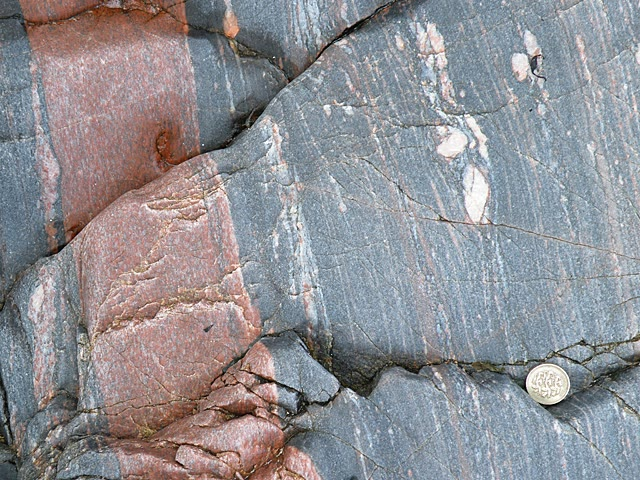
\includegraphics[width=0.5\linewidth]{images/book4/b2-12-leucogranite-vein.jpg}
\par\smallskip{\small धारीदार धूसर नाइस को काटती एक गुलाबी \omterm{def:b2:crustal-melting:leucogranite}{ल्यूकोग्रेनाइट} शिरा; सिक्का
पैमाना देता है। फ़ोटो: Anne Burgess (Geograph), CC BY-SA 2.0।}
\end{omfigure}

\section{ग्रेनाइट और महाद्वीपों की वृद्धि}\label{sec:b2:crustal-melting:time}

दो प्रकार के स्थान अधिकांश ग्रेनाइट बनाते हैं। क्षेपण क्षेत्रों के ऊपर चाप-भूपर्पटी प्रावार से आए
मैफ़िक गलितों के विभेदन से बनती है, और उपलब्ध ऊष्मा केवल उतनी है जितनी ये
गलित लाते हैं। टक्कर के बाद मोटी हुई भूपर्पटी एक बहुत गर्म तंत्र होती है: वह बड़े
पैमाने पर पिघलती है, निम्न तापमान पर जहाँ जल या मस्कोवाइट इसकी अनुमति दें और उच्चतर
तापमान पर बायोटाइट के विघटन से, और ये भूपर्पटी-व्युत्पन्न ग्रेनाइट उस भूपर्पटी का पुनर्चक्रण करते हैं जो
पहले से थी। वहाँ भी प्रावार के गलित भूपर्पटी तक पहुँचते हैं, इतनी बड़ी मात्राओं में, मोयें और
सहकर्मियों का तर्क है, कि उत्तर-पर्वतजनक पट्टियाँ भूपर्पटी की वृद्धि में महत्त्वपूर्ण योगदान देती हैं।
कोई ग्रेनाइट महाद्वीपों में कुछ जोड़ता है या केवल उन्हें पुनर्संसाधित करता है, यह इस प्रकार
उसके स्रोत का प्रश्न है, जिसका उत्तर उसके समस्थानिक देते हैं (\cref{ch:b2:isotope-geochemistry}); आरंभिक
पृथ्वी के ग्रेनाइट, जो इनसे बहुत भिन्न हैं,
\cref{ch:b2:precambrian-earth} का विषय हैं।
% ledger: moyen17:settings

\section{अभ्यास}\label{sec:b2:crustal-melting:exercises}

मोलर द्रव्यमान (\unit{\gram\per\mole}): \ce{Al2O3} 101.96, \ce{CaO} 56.08, \ce{Na2O} 61.98,
\ce{K2O} 94.20, \ce{H2O} 18.02; परमाणु द्रव्यमान: H 1.008, O 16.00, Na 22.99, Mg 24.31,
Al 26.98, Si 28.09, K 39.10, Ca 40.08। $g = \qty{9.81}{\metre\per\second\squared}$ लीजिए।

\begin{exercise}[$\star$]\label{exo:b2:crustal-melting:1}
एंडेसाइट संदर्भ पदार्थ AGV-2 में, \unit{\gram} प्रति \qty{100}{\gram} में,
\ce{Al2O3} 17.03, \ce{CaO} 5.15, \ce{Na2O} 4.204 और \ce{K2O} 2.898 हैं।
(क) उसके A/CNK और A/NK परिकलित कीजिए। (ख) उसका वर्गीकरण कीजिए, और ऐसे खनिज का नाम बताइए जिसमें उसका
अधिशेष कैल्सियम होना चाहिए।
\end{exercise}
% ledger: usgs:agv2-major

\begin{exercise}[$\star$]\label{exo:b2:crustal-melting:2}
तीन ग्रेनाइटों में, क्वार्ट्ज़ और फ़ेल्डस्पारों के अतिरिक्त, ये हैं: (क) मस्कोवाइट, बायोटाइट और गार्नेट;
(ख) हॉर्नब्लेंड, बायोटाइट और टाइटेनाइट; (ग) एजिरीन, एक सोडियम--लोहा पाइरॉक्सीन
\ce{NaFeSi2O6}, और एक सोडियमी एम्फ़ीबोल। हर एक का उसकी ऐलुमिनियम संतृप्ति से वर्गीकरण कीजिए, और बताइए
कि कौन-सा \omterm{def:b2:crustal-melting:types}{S-प्रकार का ग्रेनाइट} हो सकता है।
\end{exercise}

\begin{exercise}[$\star$]\label{exo:b2:crustal-melting:3}
\qty{2800}{\kilogram\per\cubic\metre} घनत्व वाली भूपर्पटी का रैखिक जियोथर्म
$T = \qty{10}{\celsius} + (\qty{20}{\celsius\per\kilo\metre})\,z$ है। 2 और
\qty{10}{kbar} के बीच ग्रेनाइट के आर्द्र सॉलिडस का सन्निकटन उस सरल रेखा से कीजिए जो
(\qty{680}{\celsius}, \qty{2}{kbar}) और (\qty{620}{\celsius}, \qty{10}{kbar}) से होकर जाती है। जियोथर्म उससे किस
गहराई, तापमान और दाब पर मिलता है?
\end{exercise}
% ledger: sw81:wet-solidus

\begin{exercise}[$\star$]\label{exo:b2:crustal-melting:4}
एक धूसर बायोटाइट नाइस में क्वार्ट्ज़ और फ़ेल्डस्पार की सेंटीमीटर-मोटी सफ़ेद परतें हैं, जो
उसके पर्णन के समांतर हैं, और हर एक बायोटाइट की पतली काली धारी से घिरी है; परतों के बीच
नाइस सामान्य दिखता है। (क) सफ़ेद परतों, काली धारियों और सामान्य नाइस के नाम बताइए।
(ख) चट्टान \omterm{def:b2:crustal-melting:migmatite}{मेटाटेक्साइट} है या \omterm{def:b2:crustal-melting:migmatite}{डायाटेक्साइट}, और उसकी संरचना क्या है? (ग) कुछ सौ
मीटर दूर परतें गायब हो गई हैं: एक धारीदार, ग्रेनाइट-जैसी चट्टान में नाइस की धुँधली
प्रेत-छायाएँ हैं। क्या बदल गया है?
\end{exercise}
% ledger: scmr:migmatite, bgs99:migmatite

\begin{exercise}[$\star\star$]\label{exo:b2:crustal-melting:5}
बायोटाइट को फ़्लोगोपाइट, \ce{KMg3AlSi3O10(OH)2}, मान लीजिए। (क) उसका मोलर द्रव्यमान और
वह द्रव्यमान-अंश परिकलित कीजिए जो वह जल के रूप में छोड़ता है (उसके दो हाइड्रॉक्सिल समूह एक \ce{H2O} देते हैं)।
(ख) द्रव्यमान के अनुसार \qty{25}{\percent} बायोटाइट वाला एक नाइस बायोटाइट \omterm{def:b2:crustal-melting:reactions}{निर्जलीकरण गलन} से
ऐसे गलित में पिघलता है जिसमें \qty{4.0}{\percent} जल है।
\cref{prop:b2:crustal-melting:water} का उपयोग करके \omterm{def:b2:mantle-melting:fraction}{गलन-अंश} ज्ञात कीजिए, और उसकी तुलना
बायोटाइट \omterm{def:b2:crustal-melting:reactions}{निर्जलीकरण गलन} के प्रयोगों में पाए गए अंशों से कीजिए।
\end{exercise}
% ledger: bk99:migmatites

\begin{exercise}[$\star\star$]\label{exo:b2:crustal-melting:6}
सौ ग्राम ग्रेनाइट में \qty{30}{\gram} पोटैशियम फ़ेल्डस्पार \ce{KAlSi3O8},
\qty{35}{\gram} एल्बाइट \ce{NaAlSi3O8}, \qty{5}{\gram} एनॉर्थाइट \ce{CaAl2Si2O8},
\qty{25}{\gram} क्वार्ट्ज़ और \qty{5}{\gram} मस्कोवाइट \ce{KAl3Si3O10(OH)2} हैं।
(क) चार ऐलुमिनीयुक्त खनिजों के मोलर द्रव्यमान परिकलित कीजिए। (ख) चट्टान में
\ce{Al2O3}, \ce{CaO}, \ce{Na2O} और \ce{K2O} की मात्राएँ, और उसका A/CNK, परिकलित कीजिए। (ग) कौन-सा
खनिज चट्टान को \omterm{def:b2:crustal-melting:asi}{अति-ऐलुमिनीय} बनाता है?
\end{exercise}

\begin{exercise}[$\star\star$]\label{exo:b2:crustal-melting:7}
\qty{1200}{\celsius} पर अंतर्वेधित एक बेसाल्टी \omterm{def:b2:magma-emplacement:bodies}{सिल} पूरी तरह क्रिस्टलित होकर
\qty{850}{\celsius} तक ठंडी होती है, \qty{900}{\mega\joule\per\cubic\metre} की गुप्त ऊष्मा छोड़ते हुए।
उसके चारों ओर की भूपर्पटी, \qty{650}{\celsius} पर, \qty{850}{\celsius} तक गर्म होती है और
उसका \qty{20}{\percent} पिघलता है, गलित के प्रति एकांक आयतन उसी गुप्त ऊष्मा के साथ। दोनों
चट्टानों की ऊष्मा धारिता \qty{2.5}{\mega\joule\per\cubic\metre\per\kelvin} है।
\cref{prop:b2:crustal-melting:heat} का उपयोग करके, बताइए कि एक घन मीटर बेसाल्ट कितने घन मीटर
भूपर्पटी को इस प्रकार संसाधित कर सकता है। परिणाम किन बातों की उपेक्षा करता है?
\end{exercise}
% ledger: delaney86b4:properties

\begin{exercise}[$\star\star$]\label{exo:b2:crustal-melting:8}
ऑब्सीडियन संदर्भ पदार्थ SRM 278 प्रमाणित है: \ce{Al2O3}
$14.15 \pm 0.15$, \ce{CaO} 0.983, \ce{Na2O} 4.84 और \ce{K2O} 4.16 (\unit{\percent}
द्रव्यमान के अनुसार)। (क) उसके A/CNK और A/NK परिकलित कीजिए और उसका वर्गीकरण कीजिए। (ख) \ce{Al2O3} की अनिश्चितता के दोनों
सिरों के साथ A/CNK फिर से परिकलित कीजिए। क्या वर्गीकरण दृढ़ है?
\end{exercise}
% ledger: nist278:majors

\begin{exercise}[$\star\star$]\label{exo:b2:crustal-melting:9}
\qty{800}{\celsius} पर जल से संतृप्त एक हैप्लोग्रेनाइट गलित में \qty{7.45}{\percent}
जल होता है, \qty{3}{kbar} पर, 8.94, \qty{4}{kbar} पर, 9.97, \qty{5}{kbar} पर और 13.82,
\qty{8}{kbar} पर। (क) इन चार बिंदुओं से न्यूनतम वर्गों द्वारा एक सरल रेखा समंजित कीजिए और
उसकी ढलान की तुलना प्रयोगकर्ताओं द्वारा उद्धृत \qty{1.27}{\percent} प्रति किलोबार से कीजिए।
(ख) \qty{6}{kbar} पर संतृप्ति-मात्रा का पूर्वानुमान लगाइए। (ग) गलित का वह न्यूनतम द्रव्यमान क्या है
जो \qty{6}{kbar} पर \qty{10}{\gram} जल ले जा सकता है? (घ) इस रेखा का उपयोग
\qty{15}{kbar} पर क्यों नहीं करना चाहिए?
\end{exercise}
% ledger: holtz95:solubility

\begin{exercise}[$\star\star\star$]\label{exo:b2:crustal-melting:10}
किसी मस्कोवाइट शिस्ट के निर्जलीकरण-गलन सॉलिडस का सन्निकटन उस सरल रेखा से कीजिए जो
(\qty{750}{\celsius}, \qty{6}{kbar}) और (\qty{800}{\celsius}, \qty{10}{kbar}) से होकर जाती है,
जो प्रायोगिक सीमाओं के सिरे हैं। \qty{770}{\celsius} पर एक शिस्ट
\qty{10}{kbar} से ऊष्मा पाए या खोए बिना ऊपर उठती है। (क) वह किस दाब पर
सॉलिडस तक पहुँचती है? (ख) उसके आगे उसका तापमान सॉलिडस के अनुदिश नीचे आता है, गलन के लिए ऊष्मा
उसके अपने ठंडा होने से आती है। \qty{2.5}{\mega\joule\per\cubic\metre\per\kelvin} की ऊष्मा धारिता
और \qty{900}{\mega\joule\per\cubic\metre} की गुप्त ऊष्मा के साथ, \qty{6}{kbar} तक पहुँचने पर गलित का
कितना आयतन-अंश बन चुका होता है? (ग) हिमालय के \omterm{def:b2:crustal-melting:leucogranite}{ल्यूकोग्रेनाइटों} के लिए प्रस्तावित दशाओं से
तुलना कीजिए।
\end{exercise}
% ledger: pdh98:himalaya, delaney86b4:properties

\begin{exercise}[$\star\star\star$]\label{exo:b2:crustal-melting:11}
ऊष्मा दूरी $\ell$ पर $\ell^2/\kappa$ की कोटि के समय में विसरित होती है।
$\kappa = \qty{1e-6}{\square\metre\per\second}$ के साथ, उस समय का अनुमान लगाइए जिसमें एक
\qty{2}{km} मोटी \omterm{def:b2:magma-emplacement:bodies}{सिल} की, और एक \qty{10}{km} मोटी अधःस्तरित परत की, ऊष्मा अपनी
ही मोटाई पर फैलती है। हिमालयी \omterm{def:b2:crustal-melting:anatexis}{ऐनाटेक्सिस} के दस मिलियन वर्षों से तुलना कीजिए: क्या एक
अधःस्तरण घटना इसकी व्याख्या कर सकती है?
\end{exercise}
% ledger: delaney86b4:properties, weinberg16:himalaya

\begin{exercise}[$\star\star\star$]\label{exo:b2:crustal-melting:12}
एक स्ट्रोमैटिक \omterm{def:b2:crustal-melting:migmatite}{मिग्मेटाइट} का विश्लेषण किया गया: \omterm{def:b2:crustal-melting:migmatite}{ल्यूकोसोम} \ce{K2O} \qty{5.0}{\percent}, \ce{MgO}
\qty{0.20}{\percent}; \omterm{def:b2:crustal-melting:migmatite}{मेलानोसोम} \ce{K2O} \qty{2.0}{\percent}, \ce{MgO}
\qty{4.0}{\percent}; मीसोसोम, जिसे अपिघला जनक माना गया, \ce{K2O}
\qty{2.75}{\percent}, \ce{MgO} \qty{3.05}{\percent} (सब द्रव्यमान के अनुसार)। (क) यदि
नियोसोम जनक से बिना किसी लाभ या हानि के बना, तो उसका कितना द्रव्यमान-अंश
\omterm{def:b2:crustal-melting:migmatite}{ल्यूकोसोम} है? (ख) उत्तर को \ce{MgO} से जाँचिए। (ग) अनावरण पर \omterm{def:b2:crustal-melting:migmatite}{ल्यूकोसोम} नियोसोम का केवल
\qty{10}{\percent} द्रव्यमान बनाता है। जनक चट्टान के प्रति
\qty{100}{\gram} कितने ग्राम गलित निकल गया?
\end{exercise}

\begin{problem}[{सप्ताहांत समस्या --- पिघले अभ्रक से एक प्लूटॉन}]\label{pb:b2:crustal-melting:1}
\qty{20}{\percent} मस्कोवाइट, \qty{15}{\percent} बायोटाइट,
\qty{30}{\percent} क्वार्ट्ज़, \qty{30}{\percent} प्लैजियोक्लेज़ और \qty{5}{\percent} अन्य
खनिजों (द्रव्यमान के अनुसार; एक कल्पित चट्टान) से बनी एक शिस्ट चढ़ाव से दोगुनी हुई भूपर्पटी के आधार पर स्थित है, यह
\cref{ch:b2:pt-paths} में मॉडल की गई स्थिति है। वह पिघलकर एक ग्रेनाइट \omterm{def:b2:magma-emplacement:bodies}{प्लूटॉन} को पोषित कर सकती है। आँकड़े:
अभ्यासों के आरंभ में दिए परमाणु और मोलर द्रव्यमान; ग्रेनाइट का आर्द्र सॉलिडस
(\qty{680}{\celsius}, \qty{2}{kbar}), (\qty{620}{\celsius}, \qty{10}{kbar}),
(\qty{605}{\celsius}, \qty{15.3}{kbar}) और (\qty{670}{\celsius}, \qty{27}{kbar}) से होकर जाता है;
\qty{800}{\celsius} पर ग्रेनाइटी गलित की जल-संतृप्ति मात्रा \qty{9.97}{\percent} है,
\qty{5}{kbar} पर, और \qty{13.82}{\percent}, \qty{8}{kbar} पर। मोटी हुई भूपर्पटी का मॉडल-आधार इस प्रकार चलता है:

\smallskip
\begin{center}\small
\begin{tabular}{l|ccccccccccc}
$t$ (\unit{Myr}) & 0 & 10 & 20 & 30 & 40 & 50 & 60 & 70 & 80 & 90 & 100\\ \hline
$T$ (\unit{\celsius}) & 595 & 656 & 734 & 795 & 845 & 885 & 909 & 914 & 900 & 867 & 814\\
$P$ (\unit{kbar}) & 19.2 & 19.2 & 19.2 & 19.2 & 17.9 & 16.5 & 15.1 & 13.7 & 12.4 & 11.0 & 9.6
\end{tabular}
\end{center}
\smallskip

\noindent\textbf{भाग I --- अभ्रक से जल।}
\begin{enumerate}
\item मस्कोवाइट \ce{KAl3Si3O10(OH)2} का मोलर द्रव्यमान परिकलित कीजिए।
\item उसके दो हाइड्रॉक्सिल समूह एक \ce{H2O} देते हैं। खनिज का कितना द्रव्यमान-अंश
जल के रूप में मुक्त होता है?
\item एक किलोग्राम शिस्ट का मस्कोवाइट कितना जल मुक्त करता है?
\item रैखिक अंतर्वेशन से, \qty{7}{kbar} पर गलित की संतृप्ति जल-मात्रा
क्या है? तब मस्कोवाइट का जल न्यूनतम कितना \omterm{def:b2:mantle-melting:fraction}{गलन-अंश} बना सकता है?
\item \omterm{def:b2:crustal-melting:reactions}{निर्जलीकरण गलन} का गलित संतृप्ति से बहुत दूर होता है; उसकी जल-मात्रा
\qty{6.0}{\percent} लीजिए। मस्कोवाइट कितना \omterm{def:b2:mantle-melting:fraction}{गलन-अंश} बनाता है?
\item \qty{10}{kbar} पर एक द्वि-अभ्रक \omterm{def:b2:metamorphic-facies:protoliths}{मेटापेलाइट} पर प्रयोगों में मस्कोवाइट अभिक्रिया
ने केवल 1 से \qty{2}{\percent} गलित दिया। दो कारण बताइए कि कोई वास्तविक चट्टान प्रश्न~5 के आपके उत्तर से
कम गलित क्यों बना सकती है।
\end{enumerate}

\noindent\textbf{भाग II --- स्रोत को गर्म करना।}
\begin{enumerate}[resume]
\item \cref{ch:b2:pt-paths} में मध्य-भूपर्पटी में छोड़ी गई चट्टान का शिखर \qty{593}{\celsius}
और \qty{7.8}{kbar} पर है। \qty{7.8}{kbar} पर आर्द्र सॉलिडस क्या है? क्या वह चट्टान पिघल सकती है,
मुक्त जल के साथ भी?
\item 15.3 और \qty{27}{kbar} के बीच अंतर्वेशन से, चढ़ाव के ठीक बाद आधार के दाब पर
आर्द्र सॉलिडस ज्ञात कीजिए। क्या $t = 0$ पर आधार उससे ऊपर है? $t = \qty{10}{Myr}$ पर?
\item $t = \qty{10}{Myr}$ पर आधार के गलन को क्या सीमित करता है, और वह जल्द ही
क्यों रुक जाता है?
\item आधार \qty{800}{\celsius}, यानी मस्कोवाइट सीमा का ऊपरी सिरा, कब
पार करता है?
\item एम्फ़ीबोल की सीमा 875 से \qty{925}{\celsius} तक, 10 से \qty{12.5}{kbar} पर, फैली है।
आधार इस दाब-परास में कब प्रवेश करता है, और किस तापमान पर?
\item आधार \qty{10}{kbar}, यानी मस्कोवाइट प्रयोगों के दाब-परास के ऊपरी सिरे, तक कब पहुँचता है,
और तब वह कितना गर्म है? शिस्ट के कौन-से जलयोजित खनिज अब भी
अस्तित्व में रह सकते हैं?
\end{enumerate}

\noindent\textbf{भाग III --- कौन-सा गलित?}
क्रिस्टलित होने पर गलित एक \omterm{def:b2:crustal-melting:leucogranite}{ल्यूकोग्रेनाइट} (कल्पित विश्लेषण) देता है, जिसमें
\unit{\percent} द्रव्यमान के अनुसार \ce{Al2O3} 15.0, \ce{CaO} 0.55, \ce{Na2O} 3.4 और \ce{K2O} 4.9 हैं।
\begin{enumerate}[resume]
\item चट्टान के \qty{100}{\gram} में चारों ऑक्साइडों की मात्राएँ परिकलित कीजिए।
\item उसका A/CNK परिकलित कीजिए।
\item उसका A/NK परिकलित कीजिए और \omterm{def:b2:crustal-melting:leucogranite}{ल्यूकोग्रेनाइट} का वर्गीकरण कीजिए।
\item क्या यह \omterm{def:b2:crustal-melting:types}{I-प्रकार का ग्रेनाइट} है या S-प्रकार का? ऐसे दो खनिजों के नाम बताइए जिनमें उसका अधिशेष
ऐलुमिनियम होना चाहिए।
\item फ़ेल्डस्पारों के बाद प्रति \qty{100}{\gram} \ce{Al2O3} के कितने मोल बचते हैं? यदि
वह सब मस्कोवाइट में जाए, जिसमें प्रति सूत्र-इकाई पोटैशियम फ़ेल्डस्पार से एक \ce{Al2O3} अधिक
है, तो \qty{100}{\gram} ग्रेनाइट में कितने ग्राम मस्कोवाइट
होगा?
\item ऑब्सीडियन SRM 278 का A/CNK $= 0.993$ है। क्या \omterm{def:b2:crustal-melting:leucogranite}{ल्यूकोग्रेनाइट} और ऑब्सीडियन
एक ही प्रकार के स्रोत से आ सकते हैं?
\end{enumerate}

\noindent\textbf{भाग IV --- कितनी भूपर्पटी?}
इस \omterm{def:b2:crustal-melting:leucogranite}{ल्यूकोग्रेनाइट} के एक कल्पित \omterm{def:b2:magma-emplacement:bodies}{प्लूटॉन} का आयतन \qty{1000}{\cubic\kilo\metre} है।
ग्रेनाइट के लिए \qty{2650}{\kilogram\per\cubic\metre} और
शिस्ट के लिए \qty{2800}{\kilogram\per\cubic\metre} लीजिए; मान लीजिए कि गलित का \qty{70}{\percent}
अपना स्रोत छोड़ देता है और क्रिस्टलित होते समय गलित का सारा जल निकल जाता है।
\begin{enumerate}[resume]
\item \omterm{def:b2:magma-emplacement:bodies}{प्लूटॉन} का द्रव्यमान क्या है?
\item उसके लिए गलित का कितना द्रव्यमान (अपने \qty{6.0}{\percent} जल के साथ) लगा?
\item प्रश्न~5 के \omterm{def:b2:mantle-melting:fraction}{गलन-अंश} का उपयोग करके, बताइए कि शिस्ट के कितने द्रव्यमान को पिघलना पड़ा।
\item वह शिस्ट का कितना आयतन है?
\item यदि स्रोत \qty{5}{km} मोटी एक परत था, तो वह कितने क्षेत्रफल पर पिघला?
\item इसके बजाय प्रश्न~4 के न्यूनतम \omterm{def:b2:mantle-melting:fraction}{गलन-अंश} के साथ स्रोत कितना बड़ा होता?
प्रश्न~22 से, \omterm{def:b2:magma-emplacement:bodies}{प्लूटॉन} बनाने के लिए पिघली स्रोत-भूपर्पटी का आयतन
\unit{\cubic\kilo\metre} में बताइए।
\end{enumerate}
\end{problem}
